\section{Policy Gradient Methods}
Instead of learning action-value estimates, and deriving a policy thereafter, we will now parameterize a policy directly depending on its performance. Our policy is now $\pi(a|s, \boldsymbol{\theta})$ representing the probability of taking action $a$ in state $s$ given parameter vector $\theta \in \mathbb{R}^{d'}$. \textit{Actor-critic} methods learn both a parameterised policy (the actor) and a parameterised value function estimate (the critic)

The policy parameter update is therefore
\begin{equation}
\boldsymbol{\theta}_{t+1} = \boldsymbol{\theta}_{t} + \alpha \nabla \hat{J(\boldsymbol{\theta}_{t})} 
\end{equation}

where $\hat{J(\boldsymbol{\theta}_{t})}$ is a stochastic estimate whose expectation approximates the gradient of the performance measure with respect to its argument $\boldsymbol{\theta}_{t}$.

\subsection{Policy Approximation and its Advantages}
\begin{itemize}

\item The policy can be parameterised in any way as long as $\pi(a|s, \boldsymbol{\theta})$ is differentiable.
\item If the action-space is discrete and not too large, then a natural and common kind of parameterisation is to form numerical preferences $h(s,a, \boldsymbol{\theta}) \in \mathbb{R}$ for each state-action pair. The actions with the highest preferences in each state are given the highest probabilities of being selected, for example, according to an exponential soft-max distribution:
\begin{equation}
\pi(a|s, \boldsymbol{\theta}) \doteq \frac{e^{h(s,a,\boldsymbol{\theta})}}{\sum_{b}e^{h(s,b,\boldsymbol{\theta})}}
\end{equation}.

\item We call this kind of policy parameterisation \textit{soft-max in action preferences}. An advantage of parameterising policies according to soft-max action preferences is that the approximate policy can approach a determinisitc policy, whereas with $\epsilon$-greedy action selection over action values there is always an $\epsilon$ probability of selecting a random action.
\item A second advantage of soft-max action preferences is that we can now select actions with arbritrary probabilities, rather than the greedy action selected most of the time and all other actions given probability of selection $\epsilon / |\mathcal{A}|$. This is useful in environments with imperfect information, where it is useful to act stochastically e.g. when bluffing in poker it is useful to do so randomly to unnerve an opponent.
\item Often the most important reason for using a policy-gradient method is that we can inject prior knowledge about the system in the RL agent.
\end{itemize}

\subsection{The Policy Gradient Theorem}
We define performance in the episodic case as
\begin{equation}
J(\boldsymbol{\theta}) \doteq v_{\pi\theta(s_0)},
\end{equation}
where $v_{\pi\theta(s_0)}$ is the true value function for $\pi_{\boldsymbol{\theta}}$, the policy determined by $\boldsymbol{\theta}$. And $s_0$ is some non-random start state. The policy gradient theorem then establishes that
\begin{equation} \label{eq: policy gradient theorem}
\nabla J(\boldsymbol{\theta}) \propto \sum_{s} \mu(s) \sum_{a} q_\pi(s,a) \nabla \pi(a|s, \boldsymbol{\theta})
\end{equation}

where $\mu$ is the on-policy distribution under $\pi$ as discussed previously i.e. the theorem is a sum over states weighted by how often the states occur under the target policy $\pi$. We can use this to approximate gradient ascent without access to the derivative of the state distribution.

\subsection{REINFORCE: Monte Carlo Policy Gradient}
REINFORCE is a method for updating our policy parameters based on episodic returns from states $G_t$. We update the parameters in the direction of actions that yielded highest rewards. Recall from Equation \ref{eq: policy gradient theorem} that the policy gradient theorem is a weighted sum of over states which is the same as an expectation over states:
\begin{align}
\nabla J(\boldsymbol{\theta}) &\propto \sum_{s} \mu(s) \sum_{a} q_\pi(s,a) \nabla \pi(a|s, \boldsymbol{\theta}) \\
&= \mathbb{E}_\pi \left[\sum_{a} q_\pi(S_t, a) \nabla \pi(a, S_t, \boldsymbol{\theta})  \right]
\end{align}

We can arrive at REINFORCE by replacing the sum over the random variable's possible values by an expectation under $\pi$, and then sampling the expectation. We multiply and divide the summed terms by $\pi(a | S_t, \boldsymbol{\theta})$:
\begin{align}
\nabla J(\boldsymbol{\theta}) &\propto \mathbb{E}_\pi \left[\sum_{a} \pi(a | S_t, \boldsymbol{\theta}) q_\pi(S_t, a) \frac{\nabla \pi(a, S_t, \boldsymbol{\theta})}{\pi(a, S_t, \boldsymbol{\theta})} \right] \\
&= \mathbb{E}_\pi \left[q_\pi(S_t, A_t) \frac{\nabla \pi(A_t, S_t, \boldsymbol{\theta})}{\pi(A_t, S_t, \boldsymbol{\theta})} \right] \; \; \; \text{(replacing $a$ by the sample $A_t \sim \pi$)} \\
&= \mathbb{E}_\pi \left[G_t \frac{\nabla \pi(A_t, S_t, \boldsymbol{\theta})}{\pi(A_t, S_t, \boldsymbol{\theta})} \right] \; \; \; \text{(because $\mathbb{E}_\pi \left[G_t|S_t, A_t\right] = q_\pi(S_t, A_t)$)} \\
\end{align}

The last expression is what we need: a quantity that can be sampled on each time step whose expectation is proportional to the gradient. We now arrive at the REINFORCE update
\begin{equation}
\boldsymbol{\theta}_{t+1} \doteq \boldsymbol{\theta}_{t} + \alpha G_t \frac{\nabla \pi(A_t, S_t, \boldsymbol{\theta})}{\pi(A_t, S_t, \boldsymbol{\theta})}
\end{equation}

This update makes intuitive sense. The gradient term represents the direction in parameter space that most increases the probability of taking that same action again in the future. In effect, the gradient distil the policy approximation down to the weights that were most responsible for the action taken, from there we can affect these weights based on how much we valued the action. If the action yielded high reward $G_t$, then we boost the weights in proportion to the reward, and if this action has low probability of being taken under the current policy (the denominator $\pi(A_t, S_t, \boldsymbol{\theta})$) then the weights are further boosted. Alternatively, if the action is taken often, and yields low reward, we make little adjustment to the weights, lowering their impact on the policy approximation in the long run as other weights receive boosts.

Note this is a monte carlo algorithm, using complete returns as updates, meaning it is only well defined in the episodic case, and can have high variance causing slow learning. The pseudocode for REINFORCE is given in Figure \ref{fig: 13_1}.
\begin{figure}
	\centering
	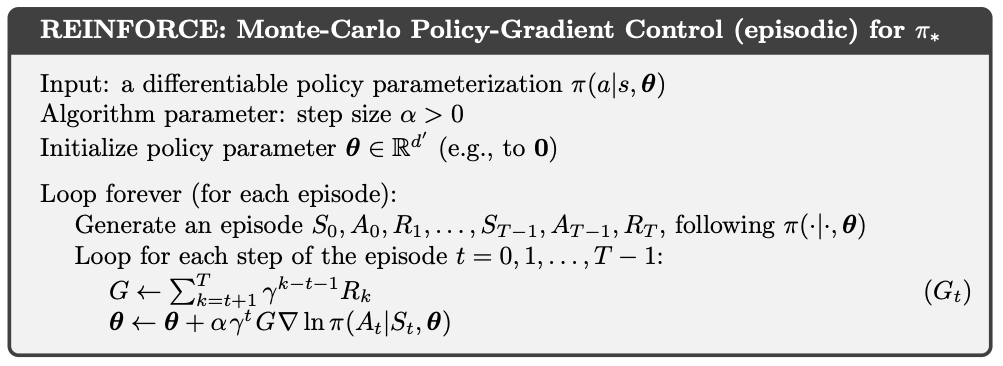
\includegraphics[width=\textwidth]{/chapter13_1}
	\caption{Pseudocode for REINFORCE: monte carlo policy-gradient control (episodic) for $\pi_*$}
	\label{fig: 13_1}
\end{figure}

\subsection{REINFORCE with Baseline}
The policy gradient theorem can be generalized to include a comparison of the action value to an arbitrary \textit{baseline} $b(s)$:
\begin{equation}
\nabla J(\boldsymbol{\theta}) \propto \sum_{s} \mu(s) \sum_{a} \left( q_\pi(s,a) - b(s) \right) \nabla \pi(a|s, \boldsymbol{\theta})
\end{equation}

We do this because it can help us reduce the variance of our results, which speeds learning. By comparing our observed result with some state-dependent baseline, we get a feel for how different the observed value is from what we expected. Thus, we arrive at a lower variance REINFORCE update as
\begin{equation}
\boldsymbol{\theta}_{t+1} \doteq \boldsymbol{\theta}_{t} + \alpha \left(G_t - b(S_t) \right) \frac{\nabla \pi(A_t, S_t, \boldsymbol{\theta})}{\pi(A_t, S_t, \boldsymbol{\theta})}
\end{equation}

The natural baseline is an estimate of the state value, $\hat{v}(S_t, \textbf{w})$, which we can learn as discussed in previous chapters. This method significantly speeds up learning as shown in Figure \ref{fig: 13_2}.
\begin{figure}
	\centering
	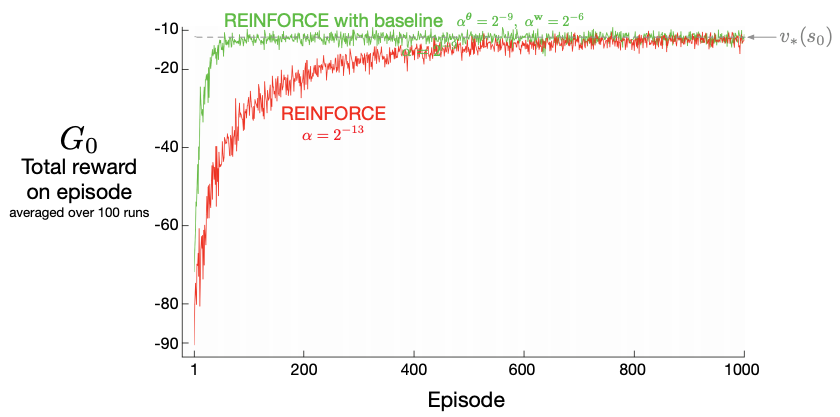
\includegraphics[width=\textwidth]{/chapter13_2}
	\caption{Adding a baseline to REINFORCE can make it learn much faster, as illustrated here on the short-corridor gridworld (Example 13.1). The step size used here for plain REINFORCE is that at which it performs best.}
	\label{fig: 13_2}
\end{figure}

\subsection{Actor-Critic Methods}
\begin{itemize}
\item The REINFORCE method uses the state-value function as a baseline for comparing true return from a state with what we expected the return to be. Because this comparison is made prior to action selection, we cannot use it to directly evaluate actions. In actor-critic methods, the state-value function is applied also to the \textit{second} state of the transition, which, when discounted and added to the one-step reward, constitutes the one-step return $G_{t:t+1}$.
\item When the state-value function is used in this way it is called the \textit{critic} and the policy is the \textit{actor}.
\item One-step actor-critic methods replace the full return of REINFORCE with the one-step return (and use a learned state-value function as the baseline) as follows:
\begin{align}
\boldsymbol{\theta}_{t+1} &\doteq \boldsymbol{\theta}_{t} + \alpha \left(G_{t:t+1} - \hat{v}(S_t, \textbf{w}) \right) \frac{\nabla \pi(A_t, S_t, \boldsymbol{\theta})}{\pi(A_t, S_t, \boldsymbol{\theta})} \\
&=  \boldsymbol{\theta}_{t} + \alpha \left(R_{t+1} + \gamma \hat{v}(S_{t+1}, \textbf{w}) - \hat{v}(S_t, \textbf{w})  \right) \frac{\nabla \pi(A_t, S_t, \boldsymbol{\theta})}{\pi(A_t, S_t, \boldsymbol{\theta})} \\
&=  \boldsymbol{\theta}_{t} + \alpha \delta_t \frac{\nabla \pi(A_t, S_t, \boldsymbol{\theta})}{\pi(A_t, S_t, \boldsymbol{\theta})} 
\end{align}
\item The pseudocode for one-step actor-critic is given in Figure \ref{fig: 13_3}, and it can be extended to include eligibility traces from Chapter 11 as shown in Figure \ref{fig: 13_4}.
\end{itemize}

\begin{figure}
	\centering
	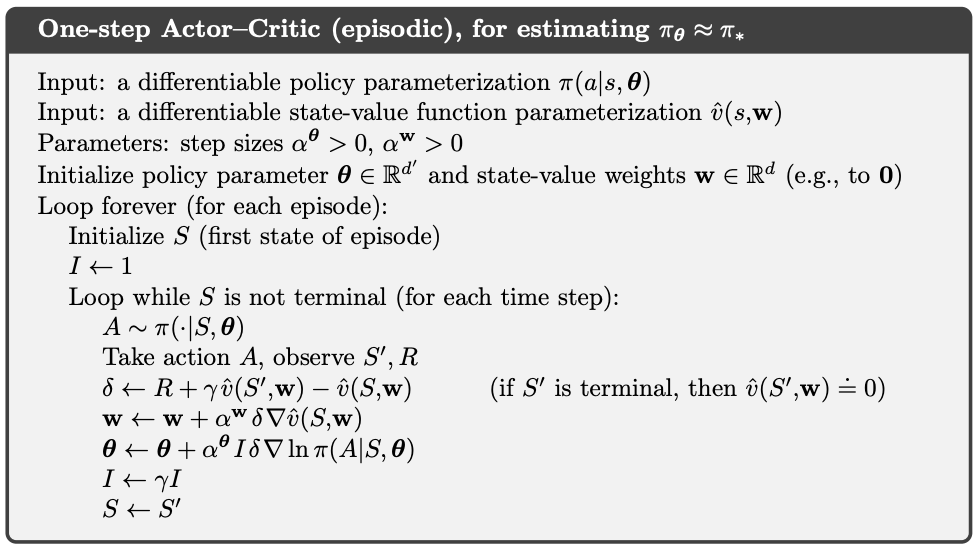
\includegraphics[width=0.8\textwidth]{/chapter13_3}
	\caption{Pseudocode for one-step actor-critic}
	\label{fig: 13_3}
\end{figure}

\begin{figure}
	\centering
	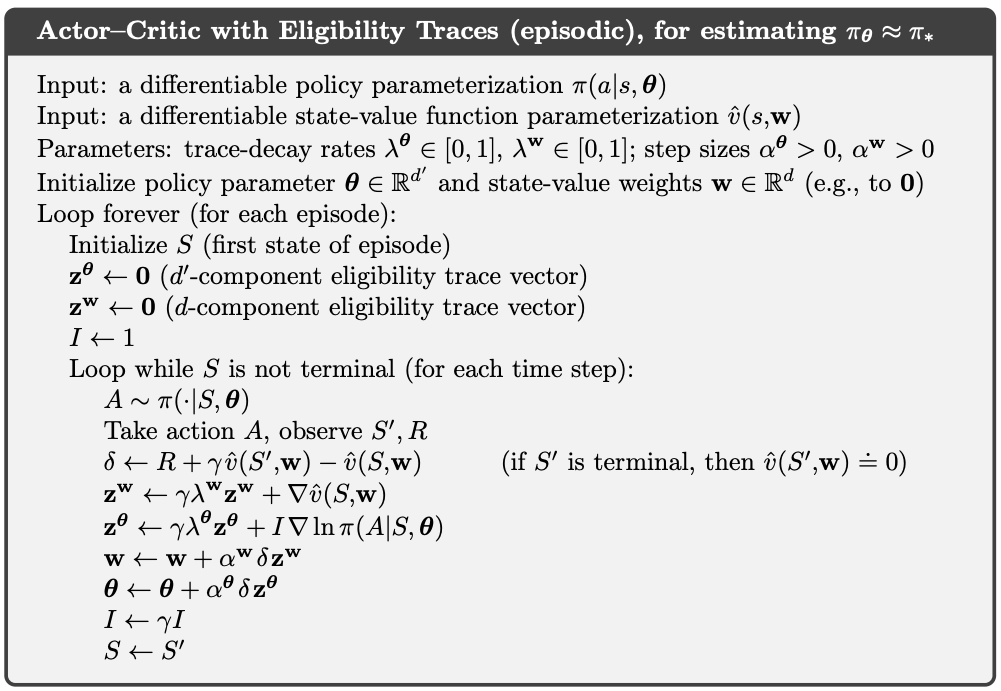
\includegraphics[width=0.8\textwidth]{/chapter13_4}
	\caption{Pseudocode for one-step actor-critic with eligibility traces}
	\label{fig: 13_4}
\end{figure}

\subsection{Policy Gradient for Continuing Problems}
As discussed in Chapter 10, for continuing problems without episode boundaries we need to define the performance in terms of average rate of reward per time step:
\begin{align}
J(\boldsymbol{\theta}) &\doteq r(\pi) \\
&= \lim_{t \rightarrow \infty} \mathbb{E} [R_t | S_0, A_{0:t-1} \sim \pi] \\
&= \sum_{s} \mu(s) \sum_{a} \pi(a | s) \sum_{s', r} p(s', r | s, a) r \\ 
\end{align}

We need to remember that in the continuing case, we define values $v_\pi(s) \doteq \mathbb{E}[G_t, S_t = s]$ and $q_\pi(s,a) \doteq \mathbb{E}[G_t, S_t = s, A_t = a]$ w.r.t the differential return:
\begin{equation}
G_t \doteq R_{t+1} - r(\pi) + R_{t+2} - r(\pi) + R_{t+3} - r(\pi) + \cdots
\end{equation}
Pseudocode for the continuing case is given in Figure \ref{fig: 13_5}.

\begin{figure}
	\centering
	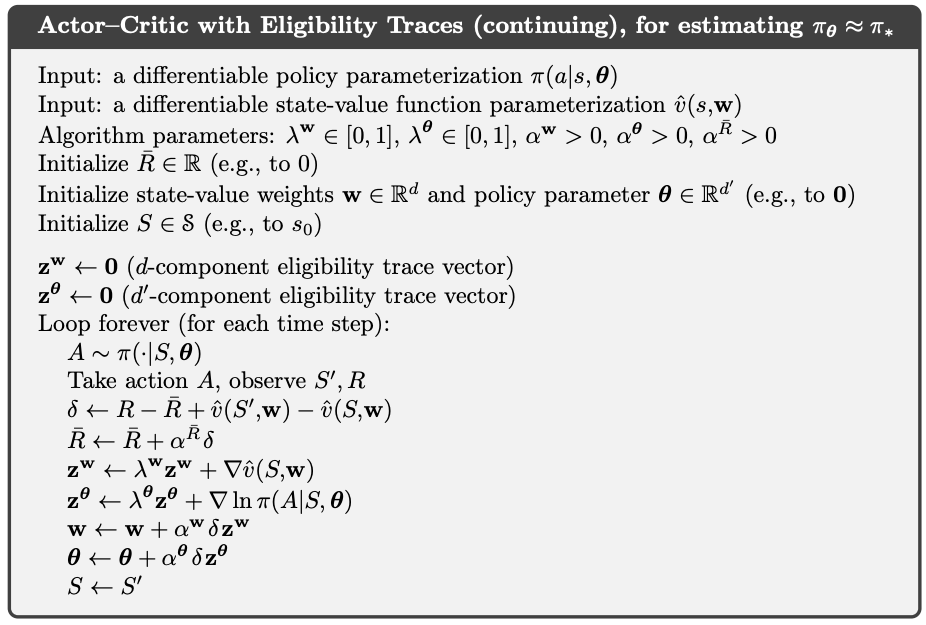
\includegraphics[width=0.8\textwidth]{/chapter13_5}
	\caption{Pseudocode for one-step actor-critic with eligibility traces, continuing case}
	\label{fig: 13_5}
\end{figure}

\subsection{Policy Parameterisation for Continuous Actions}
For state-spaces with huge numbers of actions, or continuous action spaces with infinite numbers of actions, we do not need to learn the probability of selecting each of these many actions, we can instead learn the parameters of the distribution over actions given a state. The probability density function for the normal distribution is conventionally written
\begin{equation}
p(x) \doteq \frac{1}{\sigma \sqrt{2 \pi}}exp\left(-\frac{(x - \mu)^2}{2 \sigma^2}\right)
\end{equation}

where $\mu$ and $\sigma$ are the mean and standard deviation of the normal distribution. Note $p(x)$ is the density of the probability, \textit{not} the probability itself. As such it can be greater than 1; it is the area under the graph that must sum to 1. One can take the integral between two values of $x$ to arrive at the probability of $x$ falling within that range. The policy parameterisation therefore becomes:
\begin{equation}
\pi(a | s, \boldsymbol{\theta}) \doteq \frac{1}{\sigma(s, \boldsymbol{\theta}) \sqrt{2 \pi}}exp\left(-\frac{(x - \mu(s, \boldsymbol{\theta}))^2}{2 \sigma(s, \boldsymbol{\theta})^2}\right)
\end{equation}

where $\mu : \mathcal{S} \times \mathbb{R}^{d'} \rightarrow \mathbb{R}$ and $\sigma : \mathcal{S} \times \mathbb{R}^{d'} \rightarrow \mathbb{R^+}$ i.e. they are both matrices of with dimensions equal to the number of states times the number of dimensions of the feature vector defining the policy. To from the policy approximator we need to split the policy's parameter vector into two parts, $\boldsymbol{\theta} = [\boldsymbol{\theta}_\mu, \boldsymbol{\theta}_\sigma]^T$. The mean can be approximated as a linear function, but the standard deviation must always be positive and is better approximated as the exponential of a linear function. Thus
\begin{equation}
\mu(s, \boldsymbol{\theta}) \doteq \boldsymbol{\theta}_\mu^T \textbf{x}_\mu(s) \; \; \; \text{and} \; \; \; \sigma(s, \boldsymbol{\theta}) \doteq exp\left(\boldsymbol{\theta}_\sigma^T \textbf{x}_\sigma(s)\right)
\end{equation}

\subsection{Key Takeaways}
\begin{itemize}
\item Prior to this chapter, actions had been selected by consulting an action-value function that informed us of how valuable actions were in given states at reaching our goal. Here, we instead parameterised policies directly, updating our approximations by reviewing the rewards received after taking some actions.
\item There are several advantages to doing this:
\begin{enumerate}
\item They can learn specific probabilities of taking actions (rather than sharing $\epsilon / |\mathcal{A}|)$ probability with non-greedy actions as per $\epsilon$-greedy methods)
\item They can learn appropriate levels of exploration and then approach deterministic policies in the long run
\item They can naturally handle continuous action spaces by learning distributions over actions given a state
\end{enumerate}
\item The policy gradient theorem provides a theoretical foundation for all policy gradient methods and gives an exact formula for how performance is affected by the policy parameter that does not involve derivatives of the state distribution.
\item The REINFORCE method is the policy gradient theorem in action using monte carlo returns
\item A baseline (usually our current estimate for the state-value) can be used in conjunction with REINFORCE to reduce the variance of the output and speed learning.
\item Actor-critic methods assess the policy's action selection by comparing its one-step reward with the value function at the next timestep. This introduces bias into the actor's gradient estimates, but is often desirable for the same reason that bootstrapping TD methods are often superior to Monte Carlo methods (substantially reduced variance).

\end{itemize}



